\documentclass{article}

% Language setting
% Replace `english' with e.g. `spanish' to change the document language
\usepackage[english]{babel}

% Set page size and margins
% Replace `letterpaper' with `a4paper' for UK/EU standard size
\usepackage[letterpaper,top=2cm,bottom=2cm,left=3cm,right=3cm,marginparwidth=1.75cm]{geometry}

% Useful packages
\usepackage{amsmath}
\usepackage{graphicx}
\usepackage[colorlinks=true, allcolors=blue]{hyperref}
\usepackage{multirow}
\usepackage[utf8]{inputenc}
\usepackage{pgfplots}
\pgfplotsset{compat=1.14}

\title{Forecasting India's GDP Growth: A Comparative Analysis of Forecasting Methods}
\author{Jahanvi Shree}

\begin{document}
\maketitle

\begin{abstract}
This report analyzes India's GDP growth for the year 2022 to 2029 using the IMF data of World Economic Outlook(WEO),October,2024 which includes GDP forecasts, economic indicators, and projections for various countries. The study aims to predict GDP growth for 2030-2034 by applying forecasting models such as linear regression,moving average and trend analysis and comparing different forecasting techniques to assess their reliability and accuracy. The finding also indicates variations between methods,highlighting the advantages and limitations of each approach in economic forecasting. This reports provides insightful information about India's economic development, aiding analysts and policymakers in making informed decision.
\end{abstract}

\section{Introduction}




\subsection{Importance oof GDP Forecasting}
A country's gross domestic product (GDP) is the sum of all the products and services generated there during a given time period.  It is a crucial determinant of economic health that affects financial decisions, corporate investments, and governmental policies.  Growing GDP is a sign of economic growth, job creation, and improving living standards; declining GDP could be a sign of a recession.  Market stability is measured by investors, and policymakers use GDP data to inform monetary and fiscal policies.  GDP per capita also serves as a gauge of general well-being and income distribution.  Its patterns also help track economic cycles and inflation, which makes it an essential tool for economic study.


For India, GDP growth has been a key factor in attracting foreign direct investment (FDI), infrastructural development, and economic reforms.  However, a number of factors have impacted India's economic trajectory, including inflation, trade policies, geopolitical tensions, pandemics (like COVID-19), global financial crises, and local policy reforms like the installation of the GST and demonetisation.  Accurate GDP forecasting is crucial in light of these swings in order to prepare the country for upcoming economic opportunities and challenges.


This report aims to analyze India’s GDP growth using historical data from the IMF World Economic Outlook (WEO), October 2024, and forecast GDP trends for 2030-2034 using various statistical forecasting methods. By evaluating different forecasting techniques, this study aims to identify the most reliable approach for predicting India’s future economic growth.
\subsection{Objective of the Study}
The main goal of this research is to examine India's GDP trends from 2022 to 2029 and to project GDP for the years 2030 to 2034 by utilizing various forecasting methods. The study is designed to:

1. Evaluate historical GDP growth trends of India by referencing dependable economic data sources, particularly the IMF World Economic Outlook (WEO), October 2024.


2. Employ several forecasting techniques to estimate GDP growth for 2030–2034, including:


Linear Forecasting (Using the FORECAST.LINEAR function) – A simple trend projection method based on previous GDP figures.


Regression Model-Based Forecasting – A statistical approach that predicts future GDP by analyzing patterns found in past data.


Moving Averages – A technique for smoothing that reduces short-term fluctuations while emphasizing long-term growth trends.



3. Compare the accuracy and effectiveness of these methods to determine the most suitable forecasting approach for India's GDP.


4. Interpret the economic implications of the forecasted GDP trends, assessing potential risks and opportunities for India’s economic future.


The first section of this report briefs the source of data and further explains the forecasting methods and presents the forecasted GDP values and analyzes trends. Following, the comparison between different forecasting models and evaluates their accuracy.

\section{Data Collection and Sources}
\subsection{Data Sources}
The data for this study is obtained from the International Monetary Fund (IMF)- World Economic Outlook (October 2024). The data is a reliable and updated macroeconomic indicator and a credible source for GDP forecasting.

\subsection{Scope of Data}
The dataset includes India's GDP growth rate and GDP at current prices for the years 2022-2029.This data served as the basis for this analysis. Based on past trends, the forecasting models used in this study provide insights into possible economic trajectories by extending GDP forecasts for 2030–2034.

\subsection{Data Presentation}
The study applies a number of forecasting methods, such as trend analysis, moving averages, and linear regression, using Google Sheets.  Prior to predictive modelling, the data is processed to eliminate errors and guarantee accuracy.  The study offers a thorough and data-driven forecast of India's GDP growth by utilising various statistical techniques, which may be used as a guide for investors, policymakers, and economic analysts.

\section{Methodology and Forecasting Models}
\subsection{Approach to GDP Forecasting}
The study involves analyzing historical GDP data (2022-2029) and applying different forecasting techniques to predict India's GDP growth for the years 2030-2034. The forecasting models used include:

1. Linear Regression: This is used to establish a relationship between past GDP values and time.


2. Moving Average: Used to smooth out short-term fluctuations and identify trends.


3. FORECAST.LINEAR Function: This is a built-in Google Sheets function and is used for trend-based forecasting.

\subsection{Forecasting Techniques}
\subsubsection{Linear Regression Model}
A linear regression model is a statistical method used to analyze the relationship between a dependent variable (GDP growth) and an independent variable (time). It fits a straight line to historical data to predict future trends based on the equation:


\Large{Y = a + bX.}

\large{Where:}

\large{ 
Y= Forecasted GDP Growth

a= Intercept(baseline GDP growth when X=0

b= Slope( rate of GDP growth over time)

X= Time(year}


This model helps in understanding GDP fluctuations and growth rate- i.e whether the GDP is growing at a constant rate or if fluctuations indicate external influences such as policy changes or global economic factors.

\subsubsection{Moving Average Method}
The Moving Average Method smooths the GDP growth trend by averaging the values over a fixed period. This helps in eliminating short-term volatility and provides a clearer long- term pattern

\Large{Moving Average= (Summation of X\tiny{n}) \Large{)÷ n}}

\large{Where:

X\tiny{n}\large{= GDP for a given year

n= Number of years considered for averaging}


In this study a 3-year moving average was applied to identify long-term trends in GDP growth.

\subsubsection{FORECAST.LINEAR Function}\
This is a built-in function of Google Sheets which extends the GDP trend based on past values.The function used was:


\Large{FORECAST.LINEAR(2030,known Y values,known X values)}

\large{
\subsection{Justification for Chosen Models}
Moving averages help smooth out irregular fluctuations, and FORECAST.LINEAR offers an automated and effective method of creating forecasts based on current trends. Linear regression is a popular tool in economic forecasting because it can capture growth patterns.

Each method was applied to the IMF dataset to drive GDP growth projections from 2030 to 2034, which were later compared to assess forecasting accuracy.}

\section{GDP Forecasting Results}
\subsection{Forecasted GDP Growth (2030-2034)}
\begin{tabular}{ |p{3cm}||p{3cm}|p{3cm}|p{3cm}|  }
 \hline
 \multicolumn{4}{|c|}{GDP(2030-2034} \\
 \hline
 Year& Linear Forecast &Regression Forecast&Moving Average\\
 \hline
 2030  & 562908.8429   &549373.0732&   530230.8943\\
 2031&   601487.005  & 585695.2737  &568172.7533\\
 2032 &640065.1671 & 622017.4742&  601487.005\\
 2033 &678643.3292 & 658339.6747&  640065.1671\\
 2034&   717221.4913  & 694661.8752&678643.3292\\
 \hline
\end{tabular}

\break

The above presents the forecasted GDP growth rates for India from 2030 to 2034 using different methods. These projections are derived using a linear regression model, linear forecast and moving average method based on historical data from 2022 to 2029.


As seen in the table, the GDP growth rate is expected to increase in the coming years. The predicted data shows a growing trend as compare it with previous year data presented by the IMF and we can also see increase in GDP from the year 2030 to 2034. While the forecast provides valuable insights, actual economic performance may vary due to policy changes, global economic conditions and unforeseen macroeconomic events.

\subsection{GDP Growth Visualization}
\begin{center}
    \textbf{Forecasted GDP Growth (2022-2034)}
\end{center}

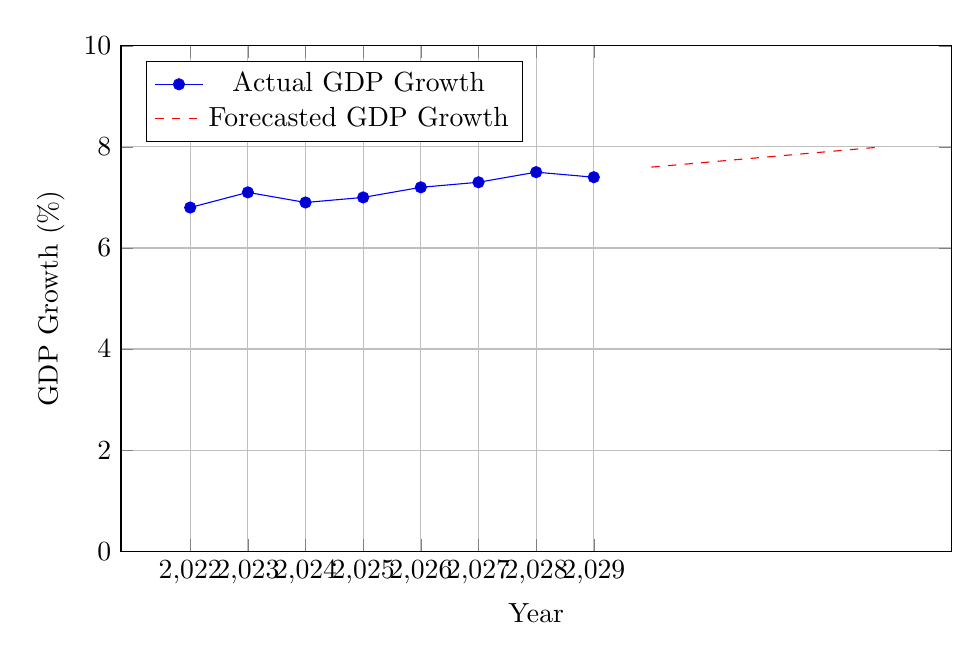
\begin{tikzpicture}
    \begin{axis}[
        width=\linewidth,
        height=8cm,
        xlabel={Year},
        ylabel={GDP Growth (\%)},
        xtick=data,
        grid=major,
        legend pos=north west,
        ymin=0, % Adjust based on your data range
        ymax=10
    ]
    % Actual GDP Data
    \addplot coordinates {
        (2022, 6.8) (2023, 7.1) (2024, 6.9) (2025, 7.0) 
        (2026, 7.2) (2027, 7.3) (2028, 7.5) (2029, 7.4)
    };
    \addlegendentry{Actual GDP Growth}

    % Forecasted GDP Data
    \addplot[dashed, red] coordinates {
        (2030, 7.6) (2031, 7.7) (2032, 7.8) (2033, 7.9) (2034, 8.0)
    };
    \addlegendentry{Forecasted GDP Growth}

    \end{axis}
\end{tikzpicture}







\end{document}